% Los anexos no tienen numeracion de seccion
\titleformat{\subsection}
	{\bfseries\large}
	{}
	{0.5pt}
	{}


\subsection{ANEXO 1: Situaci�n actual de las empresas competidoras} \label{anexo:graficos}

Los gr�ficos de las Figuras \ref{fig:inversion} y \ref{fig:presencia} han sido obtenidos de ?????.

\begin{figure}[!ht]
\centering
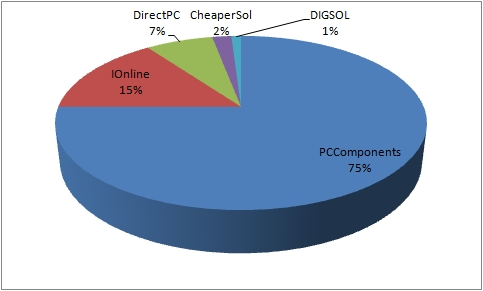
\includegraphics[scale=0.7,keepaspectratio]{./images/investigacion}%
\caption{Porcentaje de inversi�n en investigaci�n de nuevas tecnolog�as}%
\label{fig:inversion}%
\end{figure}

\begin{figure}[!ht]
\centering
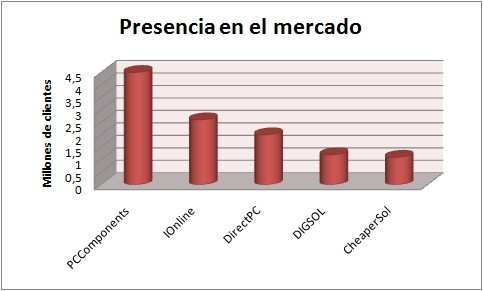
\includegraphics[scale=0.7,keepaspectratio]{./images/presencia}%
\caption{Presencia en el mercado de las empresas}%
\label{fig:presencia}%
\end{figure}

\subsection{ANEXO 2: Organigrama de la empresa DIGSOL} \label{anexo:organigrama}

\begin{spacing}{1.4}
El organigrama mostrado en la Figura \ref{fig:organigrama} ha sido cedido por el Comit� de Direcci�n de la empresa DIGSOL.
\end{spacing}

\begin{figure}[h]
\centering
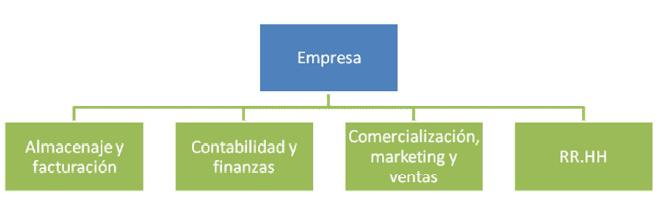
\includegraphics[scale=0.7,keepaspectratio]{./images/organigrama}%
\caption{Organigrama de la empresa DIGSOL}%
\label{fig:organigrama}%
\end{figure}


\subsection{ANEXO 3: Adquisiciones tecnol�gicas} \label{anexo:facturas}

\begin{spacing}{1.4}

Los fragmentos de facturas mostradas en las Figuras \ref{fig:factura} y \ref{fig:facturaAntigua} han sido cedidas por la Direcci�n de la empresa DIGSOL. 

La Figura \ref{fig:facturaAntigua} muestra la adquisici�n que dicha empresa realiz� a mediados del a�o 2008, cuando implant� el servicio de venta Web y actualiz� los equipos de algunos de sus departamentos.

\begin{figure}[ht]
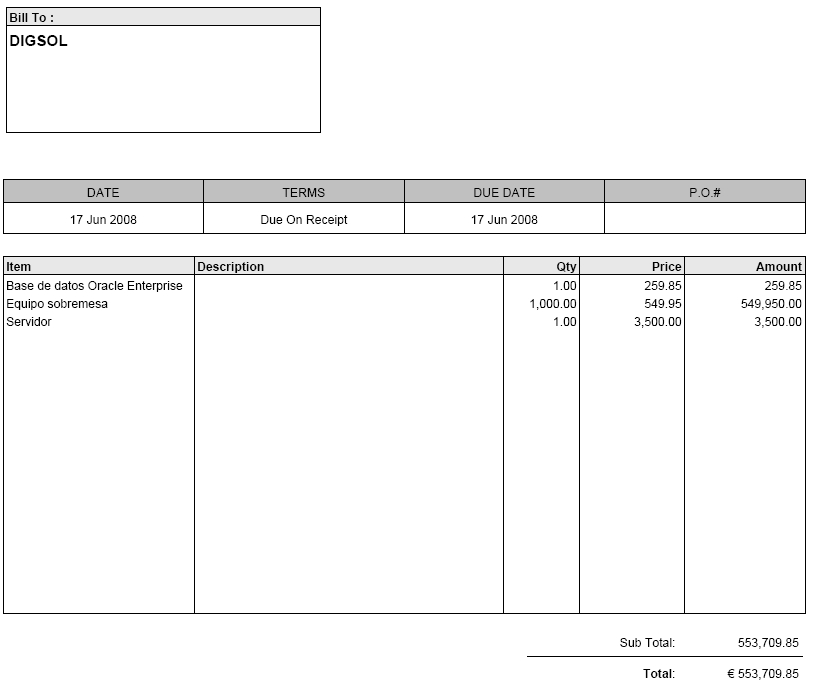
\includegraphics[scale=0.57,keepaspectratio]{./images/facturaAntigua}%
\caption{Fragmento de la factura del 17-Junio-2008}%
\label{fig:facturaAntigua}%
\end{figure}

En la factura de la Figura \ref{fig:factura} se muestra una de las �ltimas adquisiciones que ha realizado la empresa, remarcando gastos que podr�an haberse evitado (en color amarillo) y gastos totalmente innecesarios que no aportan nada de beneficio al negocio (en color rojo). 

\begin{figure}[ht]
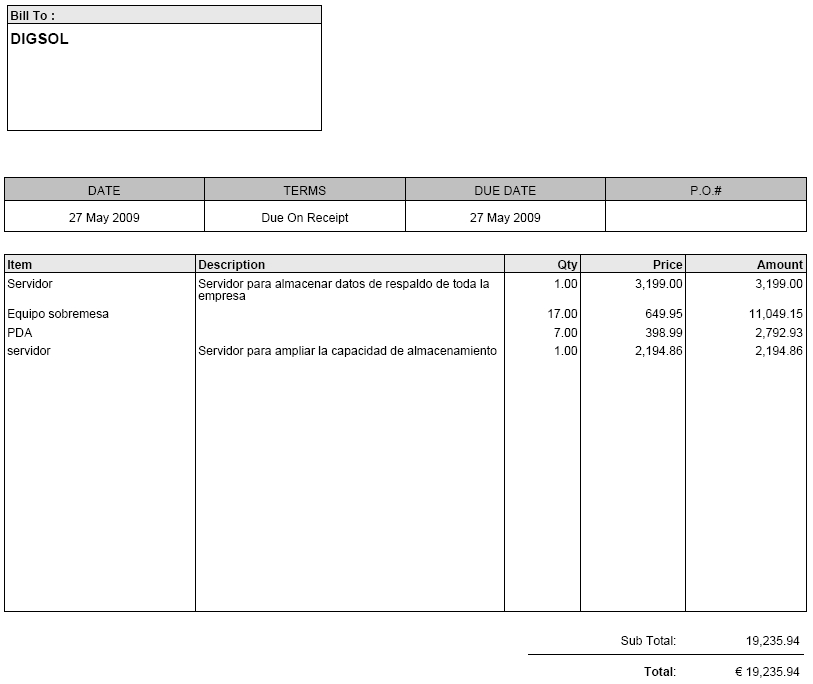
\includegraphics[scale=0.57,keepaspectratio]{./images/factura}%
\caption{Factura del 27-Mayo-2009}%
\label{fig:factura}%
\end{figure}



%El servidor de respaldo es una adquisici�n necesaria, ya que la empresa no lo renovaba desde hace unos 3 o 4 a�os. Sin embargo, la compra de los 17 equipos de sobremesa, destinados al departamento de contabilidad de la sede auditada, es algo innecesario, ya que pr�cticamente la totalidad de equipos se renovaron hace poco m�s de un a�o (coincidiendo con la implantaci�n del sistema Web), tal y como muestra la factura de esa �poca (ver Figura \ref{fig:facturaAntigua}).

%Del mismo modo, adquirir un nuevo servidor para ampliar la capacidad de almacenamiento es, en el momento actual en el que se encuentra la empresa, algo innecsario, pues el servidor que se adquiri� en su dia tiene capacidad suficiente. Podr�a pensarse entonces en qu� es una adquisici�n �til para medio o largo plazo, pero esto no es as�, ya que las tecnolog�as avanzan r�pidamente y en un plazo relativamente corto, existir�n mejores soluciones en el mercado.

%En lo que se refiere a la compra de las PDAs para las personas que integran el comit� de Direcci�n, es un gasto totalmente no justificado e in�til, ya que no se utilizan dichas PDAs para proporcionar valor al negocio. Podr�an aprovecharse para sincronizar los datos de la empresa en las PDAs, atender negocios en ella, etc., pero esto no ocurre as�.


\end{spacing}
